\paragraph{Precision vs. model}

We first provide a simple justification of the fact (used in Section~\ref{sec:sarkar}) that representing distances $d$ requires about $d$ bits in hyperbolic space -- independent of the model of the space.
Formally, we show that the number of bits needed to represent a space depends only on the maximal and minimal desired distances and the geometry of the space.
Thus although the bulk of our results are presented in the Poincar{\'e} sphere, our discussion on precision tradeoffs is fundamental to hyperbolic space.

A representation using $b$ bits can distinguish $2^b$ distinct points in a space $S$.
Suppose we wish to capture distances up to $d$ with error tolerance $\varepsilon$ -- concretely, say every point in the ball $B(0,d)$ must be within distance $\varepsilon$ of a represented point.
By a sphere covering argument, this requires at least $\frac{V_S(d)}{V_S(\varepsilon)}$ points to be represented, where $V_S(r)$ is the volume of a ball of radius $r$ in the geometry.
Thus at least $b=\log \frac{V_S(d)}{V_S(\varepsilon)}$ bits are needed for the representation.
Notice that $V_E(d) \sim d^n$ in Euclidean $\R^n$ space, so this gives the correct bit complexity of $n \log(d/\varepsilon)$.
In hyperbolic space, $V_H$ is exponential instead of polynomial in $d$, so $O(d)$ bits are needed in the representation (for any constant tolerance).
In particular, this is independent of the model of the space.


\paragraph{Graph embedding lower bound}

Now, we derive a lower bound on the bits of precision required for embedding a graph into $\mathbb{H}_2$.
Afterwards we prove a result bounding the precision for our extension of Sarkar's construction for the $r$-dimensional Poincar\'{e} ball $\mathbb{H}_r$. Finally, we give some details on the algorithm for this extension.

We derive the lower bound by exhibiting an explicit graph and lower bounding the precision needed to represent its nodes (for any embedding of the graph into $\mathbb{H}_2$). The explicit graph $G_m$ we consider consists of a root node with $\text{deg}_{\max}$ chains attached to it. Each of these chains has $m$ nodes for a total of $1+m(\text{deg}_{\max})$ nodes, as shown in Figure~\ref{fig:chains}.

\begin{figure}
\centering
\begin{minipage}[b]{0.4\textwidth}
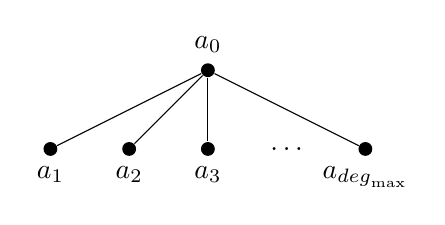
\begin{tikzpicture}[scale=1.0]
\node [circle,fill,inner sep=0pt,minimum size=5pt] (a0) at (0,1) [label={above:$a_0$}]{};
\node [circle,fill,inner sep=0pt,minimum size=5pt] (a1) at (-2,0) [label={below:$a_1$}]{};
\node [circle,fill,inner sep=0pt,minimum size=5pt] (a2) at (-1,0) [label={below:$a_2$}]{};
\node [circle,fill,inner sep=0pt,minimum size=5pt] (a3) at (0,0) [label={below:$a_3$}]{};    
\node [] (dots) at (1,0) [label={center:$\ldots$}]{};    
\node [circle,fill,inner sep=0pt,minimum size=5pt] (a4) at (2,0) [label={below:$a_{\text{deg}_{\max}}$}]{};

\draw (a0) -- (a1);
\draw (a0) -- (a2);
\draw (a0) -- (a3);
\draw (a0) -- (a4);

\end{tikzpicture}
  \end{minipage}
%  \hfill
  \begin{minipage}[b]{0.4\textwidth}
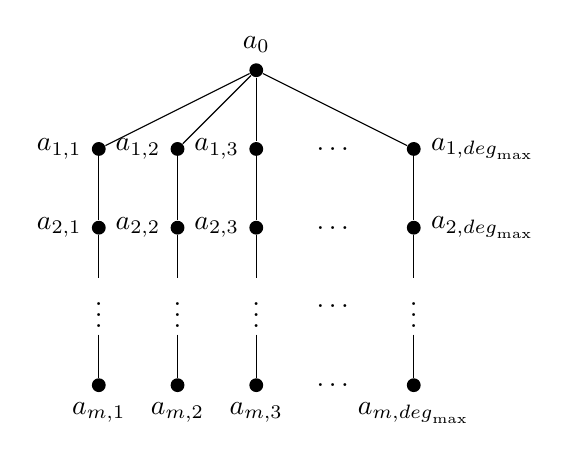
\begin{tikzpicture}[scale=1.0]
\node [circle,fill,inner sep=0pt,minimum size=5pt] (a0) at (0,1) [label={above:$a_0$}]{};
\node [circle,fill,inner sep=0pt,minimum size=5pt] (a1) at (-2,0) [label={left:$a_{1,1}$}]{};
\node [circle,fill,inner sep=0pt,minimum size=5pt] (a2) at (-1,0) [label={left:$a_{1,2}$}]{};
\node [circle,fill,inner sep=0pt,minimum size=5pt] (a3) at (0,0) [label={left:$a_{1,3}$}]{};    
\node [] (dots) at (1,0) [label={center:\ldots}]{};    
\node [circle,fill,inner sep=0pt,minimum size=5pt] (a4) at (2,0) [label={right:$a_{1,\text{deg}_{\max}}$}]{};

\node [circle,fill,inner sep=0pt,minimum size=5pt] (a5) at (-2,-1) [label={left:$a_{2,1}$}]{};
\node [circle,fill,inner sep=0pt,minimum size=5pt] (a6) at (-1,-1) [label={left:$a_{2,2}$}]{};
\node [circle,fill,inner sep=0pt,minimum size=5pt] (a7) at (0,-1) [label={left:$a_{2,3}$}]{};    
\node [] (dots2) at (1,-1) [label={center:\ldots}]{};    
\node [circle,fill,inner sep=0pt,minimum size=5pt] (a8) at (2,-1) [label={right:$a_{2,\text{deg}_{\max}}$}]{};

\node [circle,fill,inner sep=0pt,minimum size=20pt,color=white] (vdots1) at (-2,-2) [label={center:$\vdots$}]{};
\node [circle,fill,inner sep=0pt,minimum size=20pt,color=white] (vdots2) at (-1,-2) [label={center:$\vdots$}]{};
\node [circle,fill,inner sep=0pt,minimum size=20pt,color=white]  (vdots3) at (0,-2) [label={center:$\vdots$}]{};
\node [] (dots2) at (1,-2) [label={center:\ldots}]{};    
\node [circle,fill,inner sep=0pt,minimum size=20pt,color=white]  (vdots4) at (2,-2) [label={center:$\vdots$}]{};

\node [circle,fill,inner sep=0pt,minimum size=5pt] (a9) at (-2,-3) [label={below:$a_{m,1}$}]{};
\node [circle,fill,inner sep=0pt,minimum size=5pt] (a10) at (-1,-3) [label={below:$a_{m,2}$}]{};
\node [circle,fill,inner sep=0pt,minimum size=5pt] (a11) at (0,-3) [label={below:$a_{m,3}$}]{};    
\node [] (dots3) at (1,-3) [label={center:\ldots}]{};    
\node [circle,fill,inner sep=0pt,minimum size=5pt] (a12) at (2,-3) [label={below:$a_{m,\text{deg}_{\max}}$}]{};

\draw (a0) -- (a1);
\draw (a0) -- (a2);
\draw (a0) -- (a3);
\draw (a0) -- (a4);

\draw (a1) -- (a5);
\draw (a2) -- (a6);
\draw (a3) -- (a7);
\draw (a4) -- (a8);

\draw (a5) -- (vdots1);
\draw (a6) -- (vdots2);
\draw (a7) -- (vdots3);
\draw (a8) -- (vdots4);

\draw (vdots1) -- (a9);
\draw (vdots2) -- (a10);
\draw (vdots3) -- (a11);
\draw (vdots4) -- (a12);
    
\end{tikzpicture}
  \end{minipage}
\caption{Explicit graphs $G_m$ used to derive precision lower bound. Left: $m=1$ case (star graph). Right: $m>1$.}
\label{fig:chains}
\end{figure}

\begin{lemma}
The bits of precision needed to embed a graph with longest path $\ell$ is $\Omega\left(\frac{\ell}{\varepsilon} \log(\operatorname{deg}_{\max}) \right)$.
\end{lemma}
\begin{proof}



We first consider the case where $m=1$. Then $G_1$ is a star with $1+\text{deg}_{\max}$ children $a_1, a_2, \ldots, a_{\text{deg}_{\max}}$. Without loss of generality, we can place the root $a_0$ at the origin $0$. 

Let $x_i = f(a_i)$ be the embedding into $\mathbb{H}_2$ for vertex $a_i$ for $0 \leq i \leq \text{deg}_{\max}$.
We begin by showing that the distortion does not increase if we equalize the distances between the origin and each child $x_i$.
Let us write $\ell_{\max} = \max_i d_H(0,x_i) $ and $\ell_{\min} = \min_i  d_H(0,x_i)$. 

What is the worst-case distortion? We must consider the maximal expansion and the maximal contraction of graph distances.
Our graph distances are either 1 or 2, corresponding to edges ($a_0$ to $a_i$) and paths of length 2 ($a_i$ to $a_0$ to $a_j$).
By triangle inequality, $\frac{d_H(x_i,x_j)}{2} \leq \frac{d_H(0, x_i)}{2}+ \frac{d_H(0, x_j)}{2} \leq \ell_{\max}$.
This implies that the maximal expansion $\max_{i \neq j} d_H(f(a_i),f(a_j))/d_G(a_i,a_j)$ is $\frac{\ell_{\max}}{1} = \ell_{\max}$ occuring at a parent-child edge.
Similarly, the maximal contraction is at least $\frac{1}{\ell_{\min}}$. With this,
\[D_{\text{wc}}(f) \geq \frac{\ell_{\max}}{\ell_{\min}}.\]
Equalizing the origin-to-child distances (that is, taking $\ell_{\max} = \ell_{\min}$) reduces the distortion. Moreover, these distances are a function of the norms $\|x_i\|$, so we set $\|x_i\| = v$ for each child. 

Next, observe that since there are $\text{deg}_{\max}$ children to place, there exists a pair of children $x,y$ so that the angle formed by $x,0,y$ is no larger than $\theta = \frac{2\pi}{\text{deg}_{\max}}$. In order to get a worst-case distortion of $1+\varepsilon$, we need the product of the maximum expansion and maximum contraction to be no more than $1+\varepsilon$. The maximum expansion is simply $d_H(0,x)$ while the maximum contraction is $\frac{2}{d_H(x,y)}$, so we wan
\[2d_H(0,x) \leq (1+\varepsilon) d_H(x,y).\]

We use the log-based expressions for hyperbolic distance:
\[d_H(0,x) = \log \left(\frac{1+v}{1-v} \right),\]

and
\begin{align*}
d_H(x,y) &= 2 \log \left( \frac{\|x-y\| + \sqrt{\|x\|^2\|y\|^2 -2\langle x,y \rangle + 1}}{\sqrt{(1-\|x\|^2)(1-\|y\|^2)}} \right) \\
&=2 \log \left(\frac{\sqrt{2v^2(1-\cos \theta)} + \sqrt{v^4-2v^2 \cos \theta + 1}}{1-v^2} \right).
\end{align*}

This leaves us with 
\[  \log \left(\frac{\sqrt{2v^2(1-\cos \theta)} + \sqrt{v^4-2v^2 \cos \theta + 1}}{1-v^2} \right) (1+\varepsilon) \geq \log \left(\frac{1+v}{1-v} \right).\]

Now, since $1 > v^2$, we have that $\sqrt{2(1-\cos \theta)} \geq\sqrt{2v^2(1-\cos \theta)}$. Some algebra shows that  $\sqrt{3(1-\cos \theta)} \geq\sqrt{v^4 - 2v^2\cos \theta + 1}$, so that we can upper bound the left-hand side to write 
\[  \log \left(\frac{(1+\sqrt{\frac{3}{2}}) \sqrt{2(1-\cos \theta)}}{1-v^2} \right) (1+\varepsilon) \geq \log \left(\frac{1+v}{1-v} \right) .\]

Next we use the small angle approximation $\cos(\theta) = 1-\theta^2/2$ to get $\sqrt{2(1-\cos \theta)} = \theta$. Now we have
\[  \log \left(\frac{(1+\sqrt{\frac{3}{2}})  \theta }{1-v^2} \right) (1+\varepsilon) \geq \log \left(\frac{1+v}{1-v} \right) .\]

Since $v < 1$, $\frac{1}{1-v} > \frac{1}{1-v^2}$ and $\frac{1+v}{1-v} \geq \frac{1}{1-v}$, so we can upper bound the left-hand side and lower bound the right-hand side:
\[  \log \left(\frac{(1+\sqrt{\frac{3}{2}})  \theta }{1-v} \right) (1+\varepsilon) \geq  \log \left(\frac{1}{1-v} \right).\]

Rearranging,
\[ -\log(1-v) \geq -\log\left( \left(1+\sqrt{\frac{3}{2}}\right) \theta\right) \frac{1+\varepsilon}{\varepsilon}.\]

Recall that $\theta = \frac{2\pi}{\text{deg}_{\max}}$. Then we have that
\[-\log(1-v) \geq \left(\frac{1+\varepsilon}{\varepsilon} \right) \left(\log (\text{deg}_{\max}) - \log((2+\sqrt{6})\pi) \right),\]
so that
\[-\log(1-v) = \Omega\left(\frac{1}{\varepsilon} \log (\text{deg}_{\max}) \right).\]

Since $v = \|x\| = \|y\|$, $-\log(1-v)$ is precisely the required number of bits of precision, so we have our lower bound for the $m=1$ case. 

Next we analyze the $m>1$ case. Consider the embedded vertices $x_1, x_2, \ldots, x_m$ corresponding to one chain and $y_1, y_2, \ldots, y_m$ corresponding to another. There exists a pair of chains such that the angle formed by $x_m, 0, y_1$ is at most $\theta = \frac{2\pi}{\text{deg}_{\max}}$. Let $u = \|x_m\|$ and $v = \|y_1\|$. From the $m=1$ case, we have a lower bound on $-\log(1-v)$; we will now lower bound $-\log(1-u)$. The worst-case distortion we consider uses the contraction given by the path $x_m \rightarrow x_{m-1} \rightarrow \cdots \rightarrow x_1 \rightarrow 0 \rightarrow y_1$; this path has length $m+1$. The expansion is just the edge between $0$ and $y_1$. Then, to satisfy the worst-case distortion $1+\varepsilon$, we need
\[(m+1)d_H(0,y_1) \leq (1+\varepsilon)d_H(x_m,y_1).\]

Using the hyperbolic distance formulas, we can rewrite this as 
\[ 2 \log \left( \frac{\|x_m-y_1\| + \sqrt{\|x_m\|^2\|y_1\|^2 -2\langle x_m,y_1 \rangle + 1}}{\sqrt{(1-\|x_m\|^2)(1-\|y_1\|^2)}} \right) (1+\varepsilon) \geq (m+1) \log \left(\frac{1+v}{1-v} \right),\]

or,
\[ 2 \log \left( \frac{ \sqrt{u^2+v^2-2uv\cos \theta} + \sqrt{u^2v^2-2uv\cos\theta + 1}}{\sqrt{(1-u^2)(1-v^2)}} \right) (1+\varepsilon) \geq (m+1) \log \left(\frac{1+v}{1-v} \right).\]

Next,
\begin{align*}
2 \log &\left( \frac{ \sqrt{u^2+v^2-2uv\cos \theta} + \sqrt{u^2v^2-2uv\cos\theta + 1}}{\sqrt{(1-u^2)(1-v^2)}} \right) \\
 &\leq 2 \log \left( \frac{(1+\sqrt{\frac{3}{2}})\theta}{\sqrt{(1-u^2)(1-v^2)}} \right) =  \log \left( \frac{(1+\sqrt{\frac{3}{2}})^2\theta^2}{(1-u^2)(1-v^2)} \right) \\
&\leq  \log \left( \frac{(1+\sqrt{\frac{3}{2}})^2\theta^2}{(1-u)(1-v)} \right).
\end{align*}
In the first step, we used the same arguments as earlier. Applying this result and using $\frac{1+v}{1-v} \geq \frac{1}{1-v}$, we have
\[   \log \left( \frac{(1+\sqrt{\frac{3}{2}})^2\theta^2}{(1-u)(1-v)} \right)(1+\varepsilon) \geq (m+1) \log \left(\frac{1}{1-v} \right),\]
or,
\[   \log \left( \frac{(1+\sqrt{\frac{3}{2}})^2\theta^2}{1-u} \right)(1+\varepsilon) \geq (m-\varepsilon) \log \left(\frac{1}{1-v} \right).\]

Next we can apply the bound on $-\log(1-v)$.
\begin{align*}
\log\left(\frac{1}{1-u}\right) &\geq -\log\left((1+\sqrt{\frac{3}{2}})^2\theta^2\right) + \left( \frac{m-\varepsilon}{1+\varepsilon} \right) \log \left(\frac{1}{1-v} \right) \\
&\geq  -\log\left((1+\sqrt{\frac{3}{2}})^2\theta^2\right) +  \left( \frac{m-\varepsilon}{1+\varepsilon} \right) \left(\frac{1+\varepsilon}{\varepsilon} \right) \left(\log (\text{deg}_{\max}) - \log((2+\sqrt{6})\pi) \right)) \\
&= \left( \frac{m-\varepsilon}{\varepsilon} \right)  \log(\text{deg}_{\max}) - \left( \frac{m-\varepsilon}{\varepsilon} \right) \log((2+\sqrt{6})\pi) - \frac{1}{2}  \left(\log (\text{deg}_{\max}) - \log((2+\sqrt{6})\pi) \right).
\end{align*}
Here, we applied the relationship between $\theta$ and $\text{deg}_{\max}$ we derived earlier. To conclude, note that the longest path in our graph is $\ell = 2m$. Then, we have that 
\[-\log(1-u) = \Omega \left(\frac{\ell}{\varepsilon} \log(\text{deg}_{\max})\right),\]
as desired.
\end{proof}

\paragraph{Combinatorial construction upper bounds}

Next, we prove our extension of Sarkar's construction for $\mathbb{H}_r$, restated below.
 
{\bf Proposition 3.1.} \textit{The generalized $\mathbb{H}_r$ combinatorial construction has distortion at most $1+\varepsilon$ and requires at most $O(\frac{1}{\varepsilon}\frac{\ell}{r} \log \operatorname{deg}_{\max})$ bits to represent a node component for $r \leq (\log \operatorname{deg}_{\max})+1$, and $O(\frac{1}{\varepsilon}\ell)$ bits for $r > (\log \operatorname{deg}_{\max})+1$.}

\begin{proof}
%Our proof follows the lower-dimensional version of \citet{sarkar}. Briefly, the idea is that a child $Q$ is embedded in a cone emanating from parent $X$. The cone forms an angle $\alpha$, and due to the hyperbolic geometry, this angle satisfies $d_H(X,Q) = -\log \tan (\alpha/2)$. The angle $\alpha$ is determined by the degree of $X$, since we need a cone for each neighbor of $X$. Thus the degree determines the edge lengths. Moreover, to ensure $1+\varepsilon$ distortion, we take the largest such edge length $d$ and scale each edge by a common factor that ensures each edge is at least $((1+\varepsilon))/\varepsilon d$. 

The combinatorial construction achieves worst-case distortion bounded by $1+\varepsilon$ in two steps \cite{sarkar}.
First, it is necessary to scale the embedded edges by a factor of $\tau$ sufficiently large to enable each child of a parent node to be placed in a disjoint cone.
Note that there will be a cone with angle $\alpha$ less than $\frac{\pi}{\operatorname{deg}_{\max}}$.
The connection between this angle and the scaling factor $\tau$ is governed by $\tau = -\log( \tan \alpha/2)$.
As expected, as $\operatorname{deg}_{\max}$ increases, $\alpha$ decreases, and the necessary scale $\tau$ increases.

This initial step provides a Delaunay embedding (and thus a MAP of 1.0), but perhaps not sufficient distortion.
The second step is to further scale the points by a factor of $\frac{1+\varepsilon}{\varepsilon}$; this ensures the distortion upper bound. 

Our generalization to the Poincar\'{e} ball of dimension $r$ will modify the first step by showing that we can pack more children around a parent while maintaining the same angle.
In other words, for a fixed number of children we can increase the angle between them, correspondingly decreasing the scale.
We use the following generalization of cones for $\mathbb{H}_r$, defined by the maximum angle $\alpha \in [0,\pi/2]$ between the axis and any point in the cone.
Let cone $C(X,Y, \alpha)$ be the cone at point $X$ with axis $\vec{XY}$ and cone angle $\alpha$: $C(X,Y, \alpha) = \left\{ Z \in \mathbb{H}_{r} : \langle Z - X, Y - X \rangle \geq  \|Z-X\|\|Y-X\| \cos {\alpha} \right\}.$
We seek the maximum angle $\alpha$ for which $\operatorname{deg}_{\max}$ disjoint cones can be fit around a sphere.

Supposing $r-1 \le \log \operatorname{deg}_{\max}$, we use the following lower bound \cite{Jenssen} on the number of unit vectors $A(r,\theta)$ that can be placed on the unit sphere of dimension $r$ with pairwise angle at least $\theta$:
\[A(r, \theta) \geq (1+o(1)) \sqrt{2\pi r} \frac{\cos \theta}{(\sin \theta)^{r-1}}.\]

Consider taking angle
\[\theta = \asin({\operatorname{deg}_{\max}}^{-\frac{1}{r-1}}).\]
Note that
\[
  {\operatorname{deg}_{\max}}^{-\frac{1}{r-1}} = \exp \log {\operatorname{deg}_{\max}}^{-\frac{1}{r-1}} = \exp\left( -\frac{\log d}{r-1} \right) \le 1/e,
\]
which implies that $\theta$ is bounded from above and $\cos \theta$ is bounded from below.
Therefore
\[
  \operatorname{deg}_{\max} = \frac{1}{(\sin \theta)^{r-1}} \le O(1)\frac{\cos \theta}{(\sin \theta)^{r-1}} \le A(r,\theta).
\]
So it is possible to place $\operatorname{deg}_{\max}$ children around the sphere with pairwise angle $\theta$, or equivalently place $\operatorname{deg}_{\max}$ disjoint cones with cone angle $\alpha = \theta/2$.
Note the key difference compared to the two-dimensional case where $\alpha = \frac{\pi}{\operatorname{deg}_{\max}}$; here we reduce the angle's dependence on the degree by an exponent of $\frac{1}{r-1}$.

It remains to compute the explicit scaling factor $\tau$ that this angle yields; recall that $\tau = -\log( \tan \alpha/2)$ suffices~\cite{sarkar}.
We then have
% \begin{align*}
% \tau &= -\log(\tan \theta/2)  = -\log \left(\frac{\sin \theta}{1+\cos \theta} \right) = -\log \left(\frac{\sin \theta}{1 + \sqrt{1-\sin^2 \theta}} \right)\\
% &= -\log \left( \frac{1}{{\operatorname{deg}_{\max}}^{\frac{1}{r-1}} + \sqrt{{\operatorname{deg}_{\max}}^{\frac{2}{r-1}} - 1}}\right) \\ 
% &\leq  \log \left( 2\sqrt{{\operatorname{deg}_{\max}}^{\frac{2}{r-1}} - 1} \right) = \log 2 + O\left(\frac{1}{r} \log \operatorname{deg}_{\max }\right).
% \end{align*} 
\begin{align*}
  \tau &= -\log(\tan(\theta/4)) = -\log \left(\frac{\sin (\theta/2)}{1+\cos (\theta/2)} \right) = \log \left(\frac{1+\cos (\theta/2)}{\sin (\theta/2)} \right)
  \\&\le \log \left( \frac{2}{\sin(\theta/2)} \right) = \log \left( \frac{4\cos(\theta/2)}{\sin \theta} \right)
  \\&\le \log \left( \frac{4}{{\operatorname{deg}_{\max}}^{-\frac{1}{r-1}}} \right) = O\left(\frac{1}{r} \log \operatorname{deg}_{\max }\right)
  .
\end{align*}

 This quantity tells us the scaling factor without considering distortion (the first step).
 To yield the $1+\varepsilon$ distortion, we just increase the scaling by a factor of $\frac{1+\varepsilon}{\varepsilon}$.
 The longest distance in the graph is the longest path $\ell$ multiplied by this quantity.
    
Putting it all together, for a tree with longest path $\ell$, maximum degree $\operatorname{deg}_{\max}$ and distortion at most $1+\varepsilon$, the components of the embedding require (using the fact that distances $\|d\|$ require $d$ bits),
\[ O\left(      \frac{1}{\varepsilon}\frac{\ell}{r} \log d_{\max}  \right)\]
bits per component. % for $r  \leq (\log \operatorname{deg}_{\max}) + 1$.
This big-$O$ is with respect to $\operatorname{deg}_{\max}$ and any $r \le \log \operatorname{deg}_{\max} + 1$.


When $r > \log \operatorname{deg}_{\max} + 1$, $O\left( \frac{1}{\varepsilon}{\ell} \right)$ is a trivial upper bound.
Note that this cannot be improved asymptotically: As $\operatorname{deg}_{\max}$ grows, the minimum pairwise angle approaches $\pi/2$,%
\footnote{Given points $x_1, \dots, x_n$ on the unit sphere, $0 \le \| \sum x_i \|_2^2 = n + \sum_{i\neq j} \langle x_i, x_j \rangle$ implies there is a pair such that $x_i \cdot x_j \ge -\frac{1}{n-1}$, i.e. an angle bounded by $\cos^{-1}(-1/(n-1))$.}
so that $\tau = \Omega(1)$ irrespective of the dimension $r$.
% However, once we have increased the angles past $r = \log d_{\max}$ dimensions, the points cannot be further separated, and additional dimensions do not help.
\end{proof}

Next, we provide more details on the coding-theoretic child placement construction for $r$-dimensional embeddings. Recall that children are placed at the vertices of a hypercube inscribed into the unit hypersphere, with components in $\frac{\pm 1}{\sqrt{r}}$. These points are indexed by sequences ${a} \in \{0,1\}^r$ so that

\[{ x}_{ a} = \left( \frac{(-1)^{a_1}}{\sqrt{r}}, \frac{(-1)^{a_2}}{\sqrt{r}} , \ldots, \frac{(-1)^{a_r}}{\sqrt{r}} \right).\]

The Euclidean distance between ${ x}_{ a}$ and ${ x}_{ b}$ is a function of the Hamming distance $d_{\text{Hamming}}({ a},{ b})$ between ${ a}$ and ${ b}$. The Euclidean distance is exactly $2\sqrt{\frac{d_{\text{Hamming}}({ a},{ b})}{r}}$. Therefore, we can control the distances between the children by selecting a set of binary sequences with a prescribed minimum Hamming distance---a binary error-correcting code---and placing the children at the resulting hypercube vertices.

We introduce a small amount of terminology from coding theory. A binary code $\mathcal{C}$ is a set of sequences ${\bf a} \in \{0,1\}^r$. A $[r,k,h]_2$ code $\mathcal{C}$ is a binary linear code with length $r$ (i.e., the sequences are of length $r$), size $2^k$ (there are $2^k$ sequences), and minimum Hamming distance $h$ (the minimum Hamming distance between two distinct members of the code is $h$). 

The Hadamard code $\mathcal{C}$ has parameters $[2^k, k, 2^{k-1}]$. If $r=2^k$ is the dimension of the space, the Hamming distance between two members of $\mathcal{C}$ is at least $2^{k-1} = r/2$. Then, the distance between two distinct vertices of the hypercube ${ x}_{ a}$ and ${ x}_{ b}$ is $2\sqrt{\frac{r/2}{r}} = 2\sqrt{1/2} = \sqrt{2}$. Moreover, we can place up to $2^k=r$ points at least at this distance.

To build intuition, consider placing children on the unit circle ($r=2$) compared to the $r=128$-dimensional unit sphere. For $r=2$, we can place up to 4 points with pairwise distance at least $\sqrt{2}$. However, for $r=128$, we can place up to 128 children while maintaining this distance.

We briefly describe a few more practical details. Note that the Hadamard code is parametrized by $k$. To place $c+1$ children, take $k = \lceil \log_2(c+1) \rceil$. However, the desired dimension $r'$ of the embedding might be larger than the resulting code length $r=2^k$. We can deal with this by repeating the codeword. If there are $r'$ dimensions and $r|r'$, then the distance between the resulting vertices is still at least $\sqrt{2}$. Also, recall that when placing children, the parent node has already been placed. Therefore, we perform the placement using the hypercube, and rotate the hypersphere so that one of the $c+1$ placed nodes is located at this parent. 


\paragraph{Embedding the ancestor transitive closure}
Prior work embeds the transitive closure of the WordNet noun hypernym graph \cite{fb}. Here, edges are placed between each word and its hypernym ancestors; MAP is computed over edges of the form (word, hypernym), or, equivalently, edges $(a,b)$ where $b\in \mathcal{A}(a)$ is an ancestor of $a$.

In this section, we show how to achieve arbitrarily good MAP on these types of transitive closures of a tree by embedding a weighted version of the tree (which we can do using the combinatorial construction with arbitrarily low distortion for any number dimensions). The weights are simply selected to ensure that nodes are always nearer to their ancestors than to any other node.

Let $T = (V,E)$ be our original graph. We recursively produce a weighted version of the graph called $T'$ that satisfies the desired property. Let $s$ be the depth of node $a \in V$. We weight each of the edges $(a,c)$, where $c$ is a child of $a$ with weight $2^s$. Now we show the following property: 

\begin{proposition}
Let $b \in \mathcal{A}(a)$ be an ancestor of $a$ and $e \not\in \mathcal{A}(a)$ be some node not an ancestor of $a$. Then,
\[d_G(a,b) < d_G(a,e).\]
\end{proposition}
\begin{proof}
Let $a$ be at depth $s$. First, the farthest ancestor from $a$ is the root, at distance $2^{s-1}+2^{s-2}+ \ldots + 2+1 = 2^s-1$. Thus $d_G(a,b) \leq 2^s-1$. 

If $e$ is a descendant of $a$, then $d_G(a,e)$ is at least $2^s$ Next, if $e$ is neither a descendant nor an ancestor of $a$, let $f$ be their nearest common ancestor, and let the depths of $a,e,f$ be $s,s_2,s_3$, respectively, where $s_3 < \min\{s_1,s_2\}$. We have that 
\begin{align*}
d_G(a,e) &= (2^{s-1}+\ldots+2^{s_3}) + (2^{s_2-1} + \ldots+2^{s_3}) \\
&= 2^{s} - 2^{s_3} + 2^{s_2} - 2^{s_3} \\
&=2^{s} + 2^{s_2} - 2^{s_3+1} \\
&\geq 2^{s} \\
&> d_G(a,b).
\end{align*}
The fourth line follows from $s_2 > s_3$. This concludes the argument.
\end{proof}

Therefore, embedding the weighted tree $T'$ with the combinatorial construction enables us to keep all of a word's ancestors nearer to it than any other word. This enables us to embed a transitive closure hierarchy (like WordNet's) while still embedding a nearly tree-like graph.
\footnote{Note that further separation can be achieved by picking weights with a base larger than $2$.}
Furthermore, the desirable properties of the construction still carry through (perfect MAP on trees, linear-time, etc).



%%% Local Variables:
%%% mode: latex
%%% TeX-master: "hyperbolic_arxiv"
%%% End:
